Start de Hyper-V manager als Administrator zodat je voldoende rechten hebt om VMs aan te maken (zie \ref{HV_man_start}
\begin{figure}[H]
	\centering
	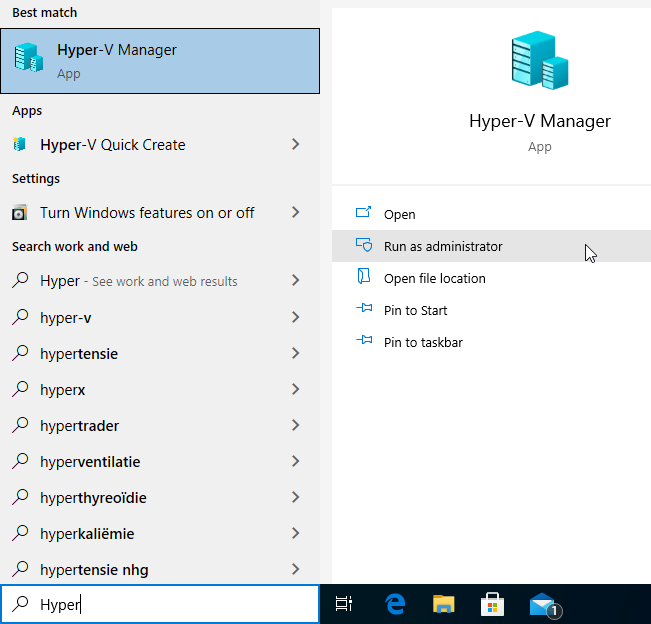
\includegraphics{hyperv_manager_start.png}
	\caption{Hyper-V Manager opstarten}
	\label{HV_man_start}
\end{figure}

Selecteer de server waaraan de manager moet connecten. In de voorbeelden wordt gebruik gemaakt van de Windows 10 desktop machine waarop we Hyper-V ge\"installeerd hebben. De hostname is zichtbaar in de linker kolom (zie \ref{HV_man_server}
\begin{figure}[H]
	\centering
	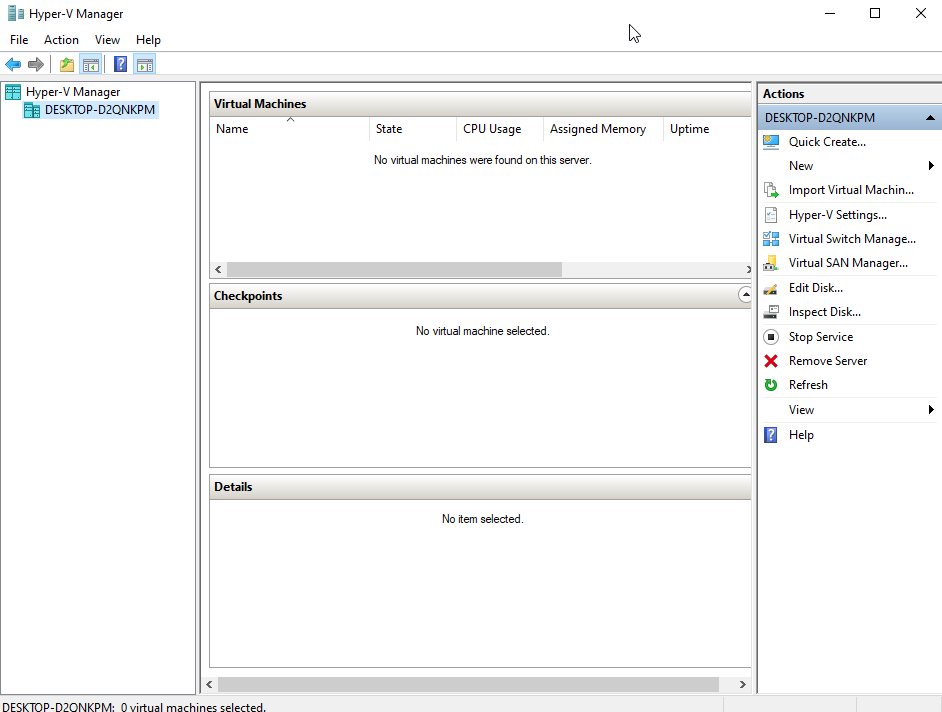
\includegraphics[width=\linewidth]{hyperv_manager_server.png}
	\caption{Hyper-V selecteer de hypervisor die je wil managen}
	\label{HV_man_server}
\end{figure}

Aan de rechterkant selecteer de New (\ref{HV_man_vm_new}) optie en kies Virtual Machine...
\begin{figure}[H]
	\centering
	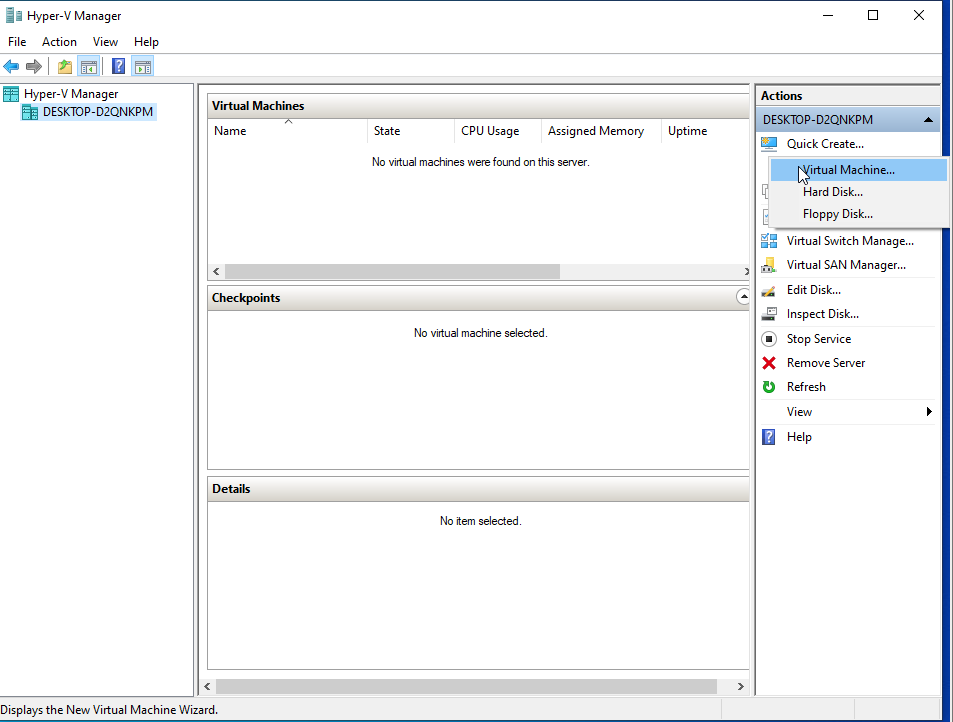
\includegraphics[width=\linewidth]{hyperv_manager_vm_new.png}
	\caption{Hyper-V installatie}
	\label{HV_man_vm_new}
\end{figure}

De eerste pagina is een introductie zoals te zien is in \ref{HV_vmnew_begin}.
\begin{figure}[H]
	\centering
	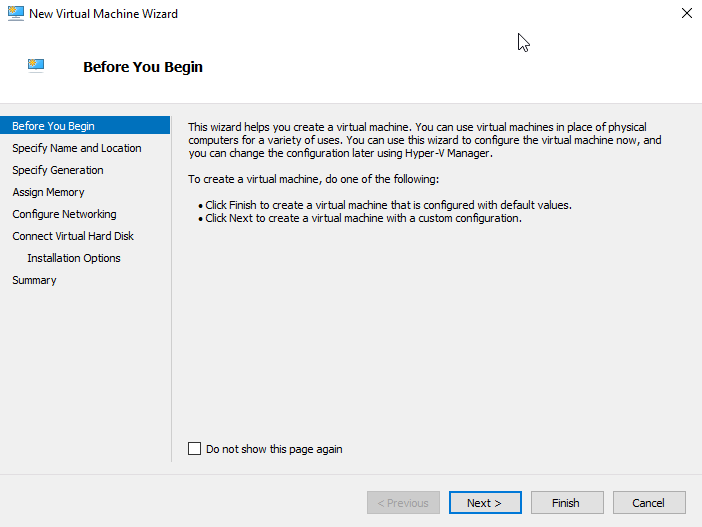
\includegraphics{hyperv_vmnew_begin.png}
	\caption{Hyper-V de begin pagina voor het maken van een nieuwe VM}
	\label{HV_vmnew_begin}
\end{figure}

Na het klikken op Next kom je in het volgende scherm terecht waar we de machine een naam gaan geven (\ref{HV_vmnew_name}
\begin{figure}[H]
	\centering
	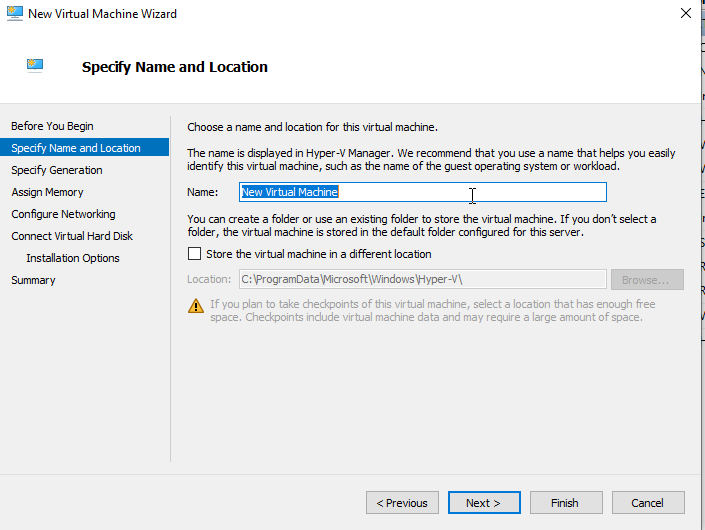
\includegraphics{hyperv_vmnew_name.png}
	\caption{Hyper-V geef de VM een naam}
	\label{HV_vmnew_name}
\end{figure}

Selecteer de generatie. De beschrijving geeft al aan dat Generatie 1 32- en 64-bits systemen kan doen en Generatie 2 alleen 64-bits systemen (\ref{HV_vmnew_gen}
\begin{figure}[H]
	\centering
	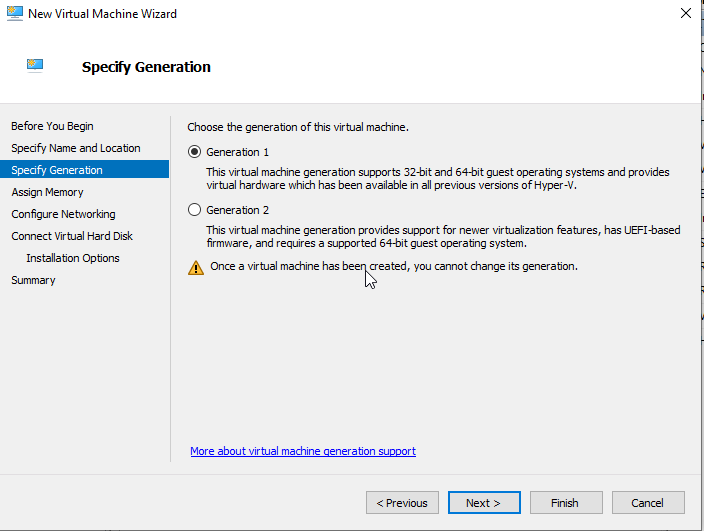
\includegraphics{hyperv_vmnew_gen.png}
	\caption{Hyper-V selecteer de VM generatie}
	\label{HV_vmnew_gen}
\end{figure}

Daarna moeten we bepalen hoeveel RAM deze virtuele machine mag gebruiken \ref{HV_vmnew_ram}
\begin{figure}[H]
	\centering
	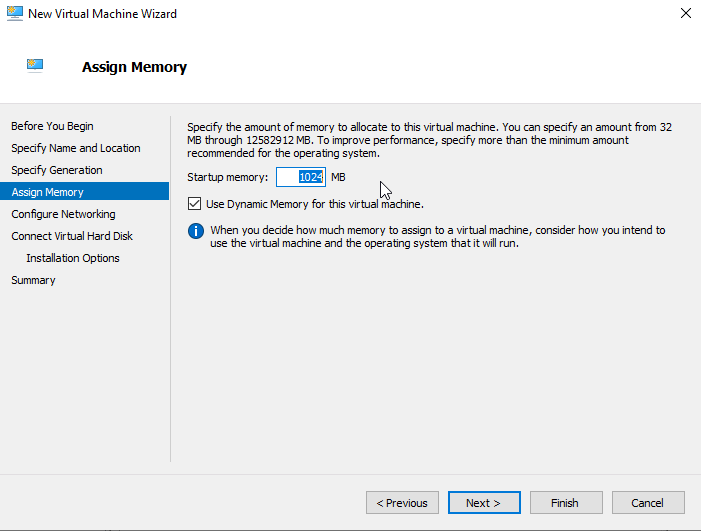
\includegraphics{hyperv_vmnew_ram.png}
	\caption{Hyper-V kies de hoeveelheid RAM voor je VM}
	\label{HV_vmnew_ram}
\end{figure}

Voor de netwerk configuratie is er een nieuwe installatie van Hyper-V alleen het default netwerk aanwezig (\ref{HV_vmnew_net}. Het aanmaken van nieuwe netwerken wordt in een volgende paragraaf besproken.
\begin{figure}[H]
	\centering
	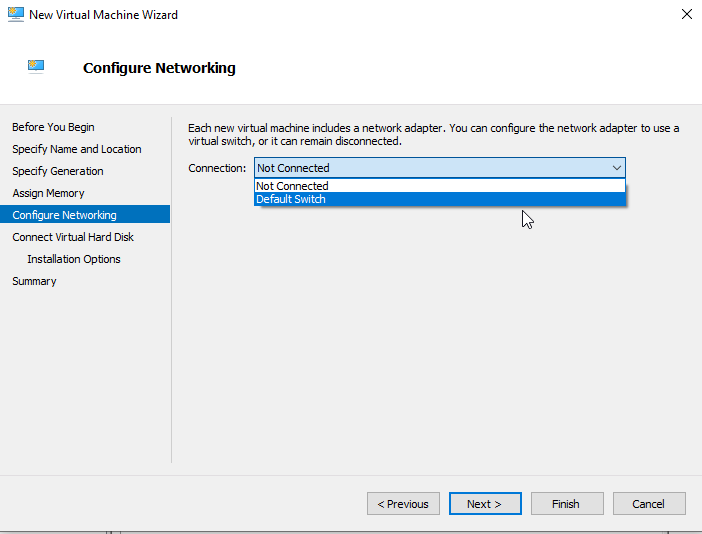
\includegraphics{hyperv_vmnew_net.png}
	\caption{Hyper-V netwerk configuratie}
	\label{HV_vmnew_net}
\end{figure}

We moeten in figuur \ref{HV_vmnew_hd} bepalen hoe groot de harddisk moet worden.
\begin{figure}[H]
	\centering
	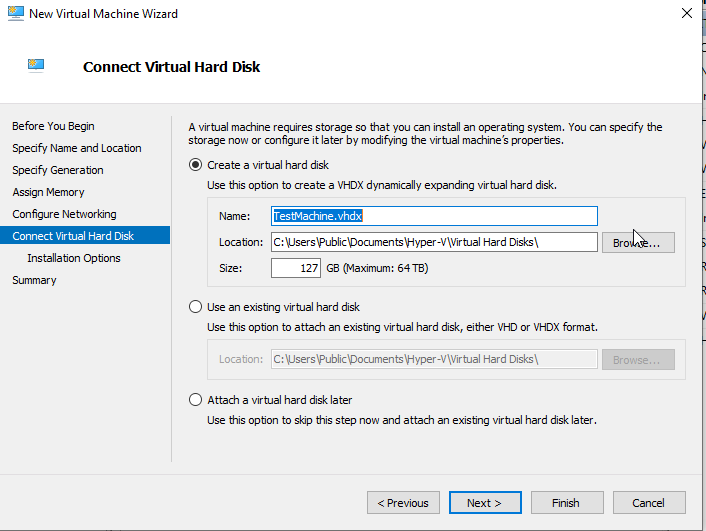
\includegraphics{hyperv_vmnew_hd.png}
	\caption{Hyper-V Harddisk configuratie}
	\label{HV_vmnew_hd}
\end{figure}

Bij Hyper-V krijgen we bij het aanmaken van een VM de vraag of we een OS willen installeren en zo ja waar deze vandaan moet komen. We kunnen selecteren om het systeem op te starten vanaf een ISO-image (\ref{HV_vmnew_os}.
\begin{figure}[H]
	\centering
	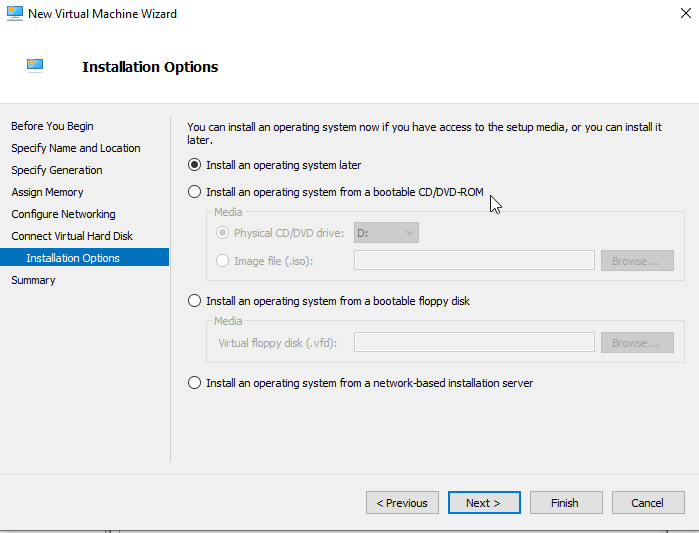
\includegraphics{hyperv_vmnew_osinst.png}
	\caption{Hyper-V Bepaal hoe je een OS op de VM gaat installeren}
	\label{HV_vmnew_os}
\end{figure}

Tenslotte krijg je een overzicht met de gekozen opties en kan je via Finish de creatie van de VM voltooien (\ref{HV_vmnew_finish}
\begin{figure}[H]
	\centering
	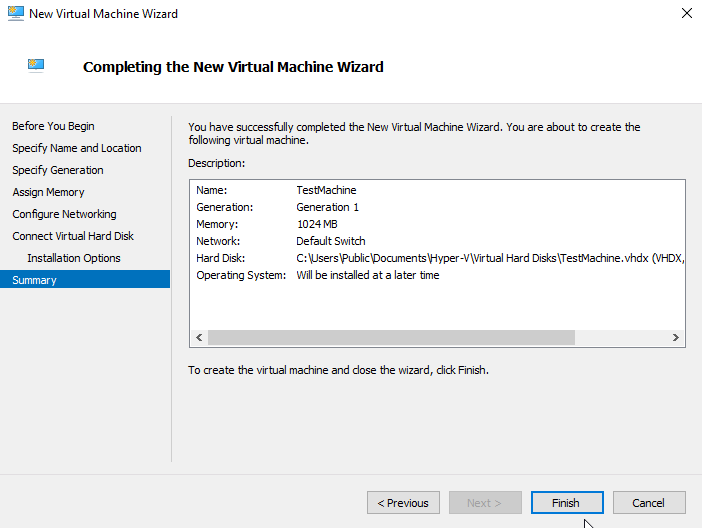
\includegraphics{hyperv_vmnew_summ.png}
	\caption{Hyper-V het daadwerkelijk aanmaken van de VM}
	\label{HV_vmnew_finish}
\end{figure}

